%!TEX root = ../dissertation.tex

\chapter{Kerbero}
\label{cap:four}
\newthought{This chapter outlines} design and implementation choices about the project in which I had worked during my internship with Kuama Srl. The project is called Kerbero and it is a new application which provides one-point access for multiple smart-lock devices. In addition, it is strongly oriented toward the check-in and check-out of users of the vacation rental system. The application aims to integrate with these platforms, in order to provide the possibility to create a temporary key for the guests, which expires at the end of their stay. Moreover, the application should be compliant with the highest number of open \acrshort{api}s for smart-locks. In order to do that, an architecture must be implemented that can interface with multiple plugins for each of the devices that the goal is to support.
\\ Continuing, we discuss the initial requirement analysis; the feasibility study and the first tests on the technologies chosen; a discussion on the design choices about how to model the concept of keys for the guest, how to manage the identity of an host in the system and how to authenticate.

\section{Requirements analysis}
The initial phase of the project involves many meetings with the committer. Being Kerbero an internal project, the committer was my tutor, with whom we defined all the requirements and the use cases of the application. As such, all the use cases and requirements are retrieved, updated and documented during the whole project, thanks to the continuous interaction between developers and committer. 
In this section, the whole requirement analysis is not reported, but only the use cases and scenarios useful to understand the choices we made during the design of the architecture and the choice of technologies are reported. As such, this analysis results being more discursive and less formal.

\subsection{Actors}
\label{sec:actors}
First of all, we defined the roles involved in the use of the application. During the analysis, we found that the application is strongly oriented towards the host "actor". The idea composed around the project foresees that the host is the actual user which, once logged in, can have access to the application features. 
However, we later realized that guests also need a way to interact. In fact, they have to receive an actual virtual key with which they can lock or unlock the smart-lock.
\\ Finally, we realize that only the host needs an identification within the system. As such, we decided to have the ease approach for the guests, which foresees that they should not have to register any account. 
\begin{figure}[H]
    \centering
    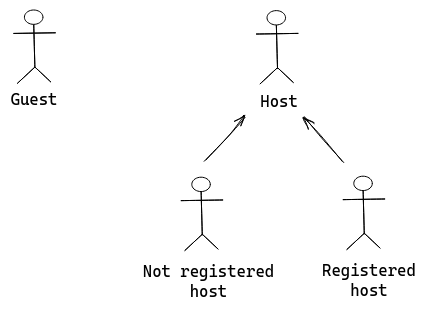
\includegraphics[width=0.5\textwidth]{figures/actors.excalidraw.png}
    \caption{Actors scheme from the requirements analysis}
    \label{fig:requirementactors}
\end{figure}
In light of the previous considerations, the identified actors are the following (fig. \ref{fig:requirementactors}):
\begin{itemize}
    \item the guest, which does only own a key and can open and close the door;
    \item the not authenticated host, which has the possibility to register an account or log with an already existing one;
    \item the authenticated host, indeed, has all the permissions, as such he can have access to all the features of the application.
\end{itemize}

\subsection{Use cases}
In order to analyze the requirements defined by the committer, it is best practice to produce use cases. Use cases are usually represented by UML diagrams and define the interaction of the actors with the system.
\\ The definition of use cases was made top-down and, as such, we first define the main features and then refine them step by step.
\subsubsection{General}
\begin{figure}[H]
    \centering
    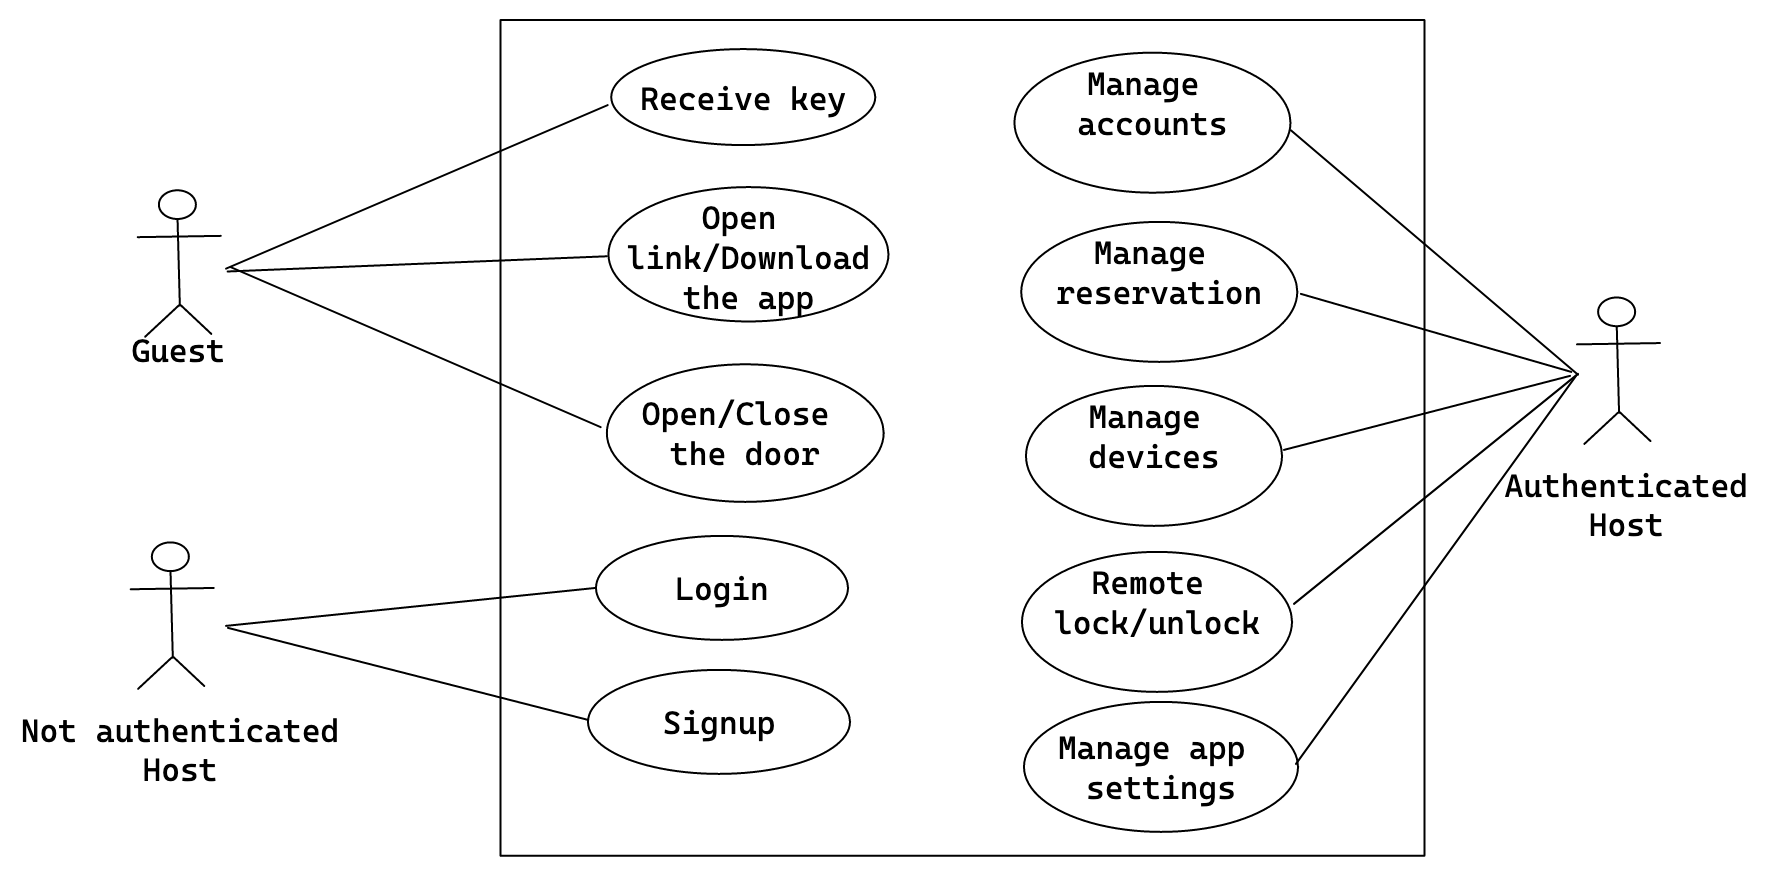
\includegraphics[width=0.9\textwidth]{figures/general.excalidraw.png}
    \caption{General use case}
    \label{fig:generalusecase}
\end{figure}
Starting from the highest level, the general use case defines the main features that we identify to be implemented in the application, giving an abstract idea of what the application must do. 
\\ First of all, there are all the features related to authentication and identity. In particular, a not authenticated host can sign up and login, while an authenticated one can sign out.
\\ After that, a guest is able to receive a key and through a link opens a page from which he can lock and unlock the smart-lock.
\\ Furthermore, an authenticated host can access the main feature of the application, which are:
\begin{itemize}
    \item manage the smart-lock provider accounts (e.g. add/remove a Nuki account);
    \item manage the reservations, manually add guests details, arrival and departure time, in order to create the correct keys;
    \item manage the devices, downloaded from the linked accounts;
    \item remote lock and unlock the smart-locks;
    \item manage the app settings.
\end{itemize}

\subsubsection{Authentication}
\begin{figure}[H]
    \centering
    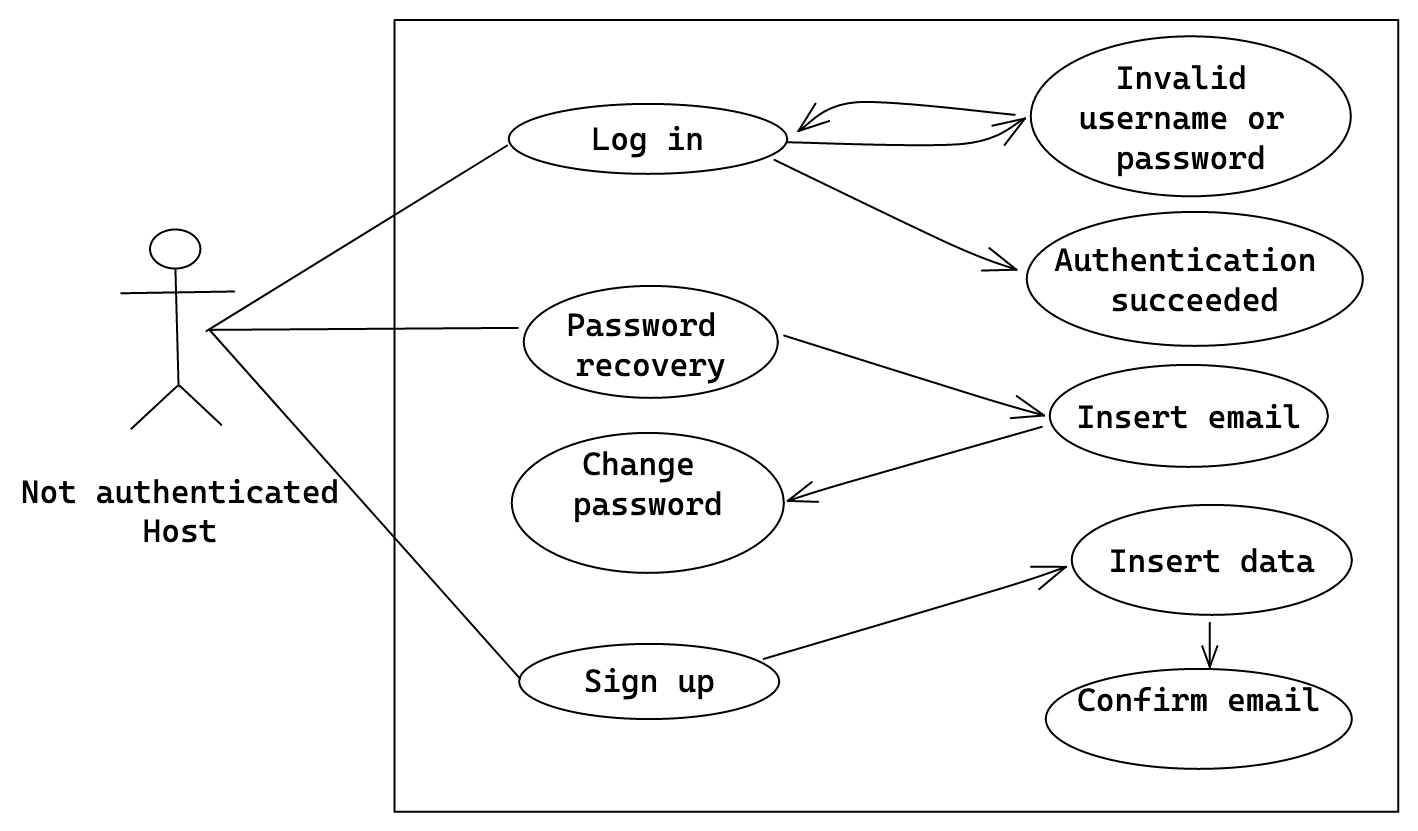
\includegraphics[width=0.9\textwidth]{figures/authentication.excalidraw.png}
    \caption{Authentication use case}
    \label{fig:authenticationusecase}
\end{figure}
The authentication is managed with a common log in and sign up system. Moreover, since account management (known as sign-up) is entrusted to the user, there is the possibility to recover the account if the user has forgotten the credentials. 

\subsubsection{Smart-lock accounts management}
\begin{figure}[H]
    \centering
    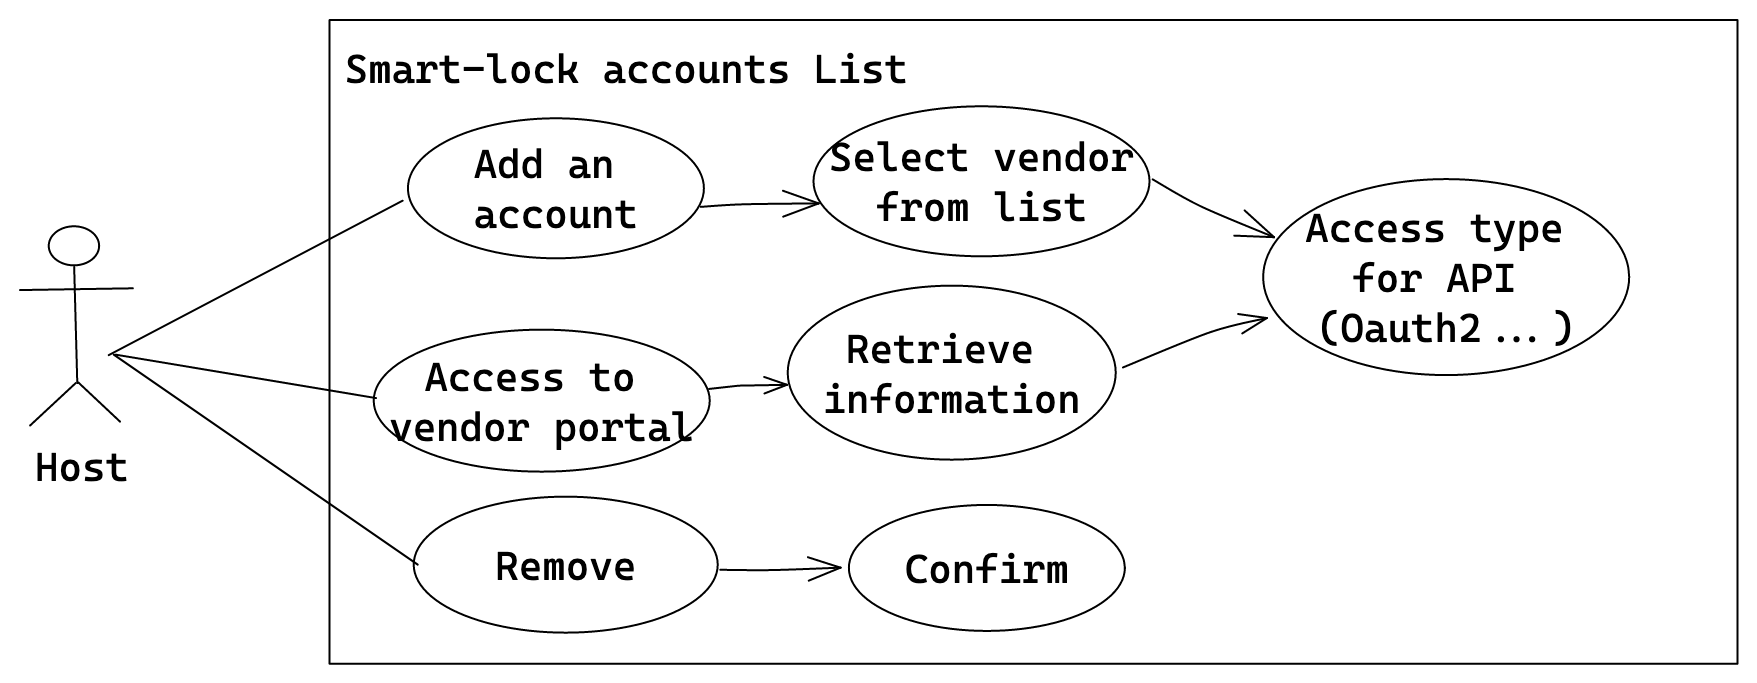
\includegraphics[width=0.8\textwidth]{figures/accounts.excalidraw.png}
    \caption{Smart-lock accounts management use case}
    \label{fig:accountsusecase}
\end{figure}
The authenticated host must be able to add a new smart-lock provider account. This integration with the external account should synchronize the information. He can remove a selected account as well.
\subsubsection{Devices management}
\begin{figure}[H]
    \centering
    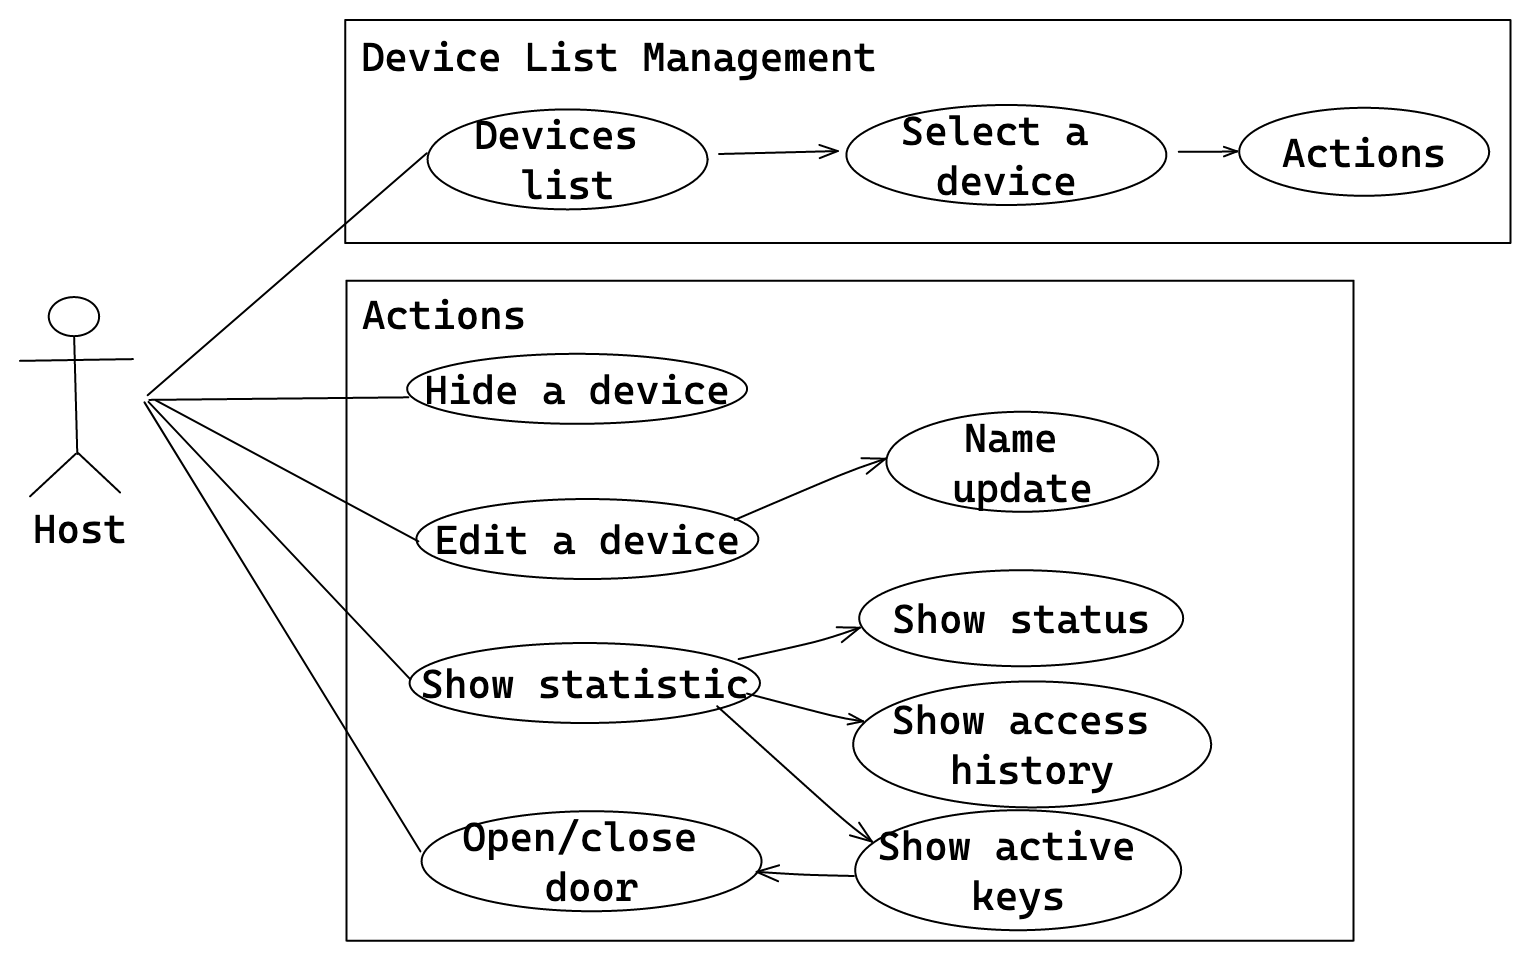
\includegraphics[width=0.8\textwidth]{figures/devices.excalidraw.png}
    \caption{User devices use case}
    \label{fig:deviceusecase}
\end{figure}
We decided to give the host the ability to see the list of devices synchronized with the provider accounts. Moreover, it is possible to lock and unlock, edit and show a status page for each of them.
\subsubsection{Keys management}
\begin{figure}[H]
    \centering
    \begin{subfigure}[b]{\textwidth}
        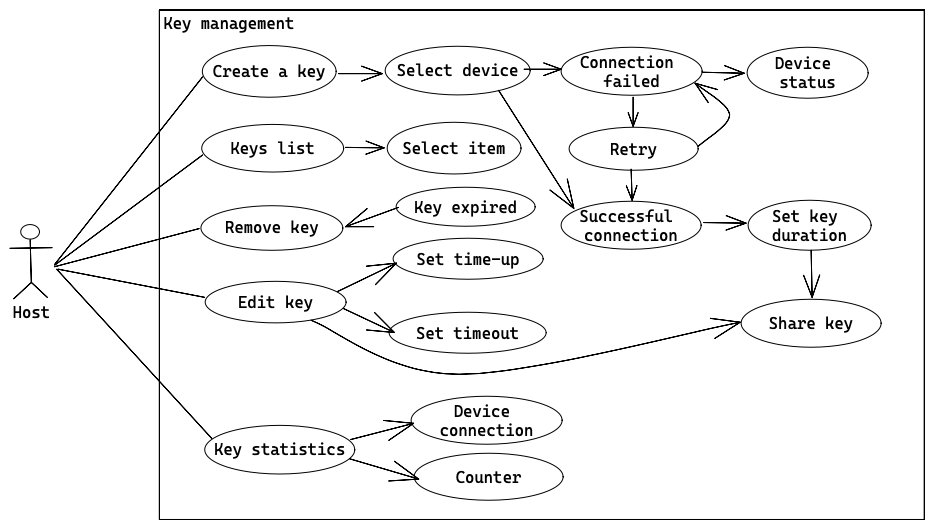
\includegraphics[width=\textwidth]{figures/keys.excalidraw.png}
    \end{subfigure}
    \begin{subfigure}[b]{\textwidth}
        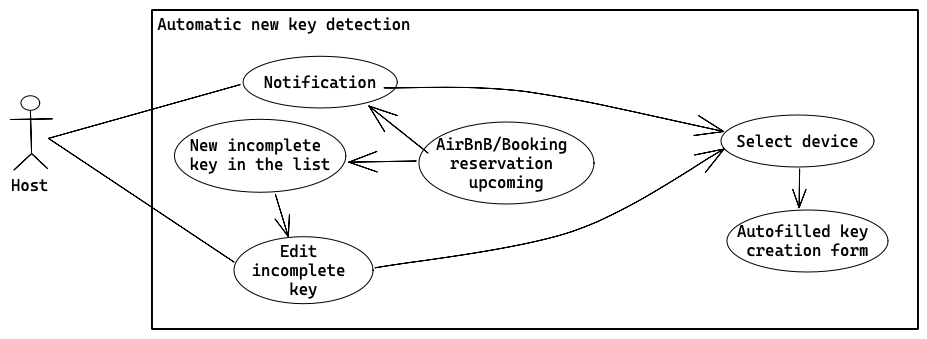
\includegraphics[width=\textwidth]{figures/autokey.excalidraw.png}
    \end{subfigure}
    \begin{subfigure}[b]{\textwidth}
        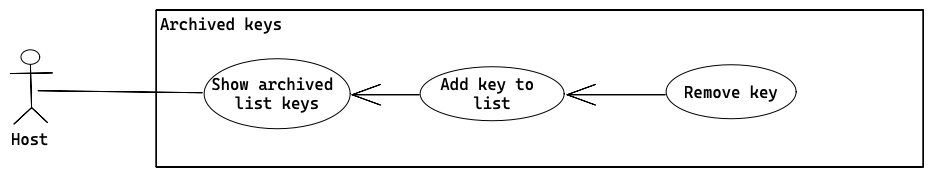
\includegraphics[width=\textwidth]{figures/keylist.excalidraw.png}
    \end{subfigure}
    \caption{Key use case, with automatic creation from reservation and key archive}
    \label{fig:keyusecases}
\end{figure}
The management of virtual keys is the core feature of the application. The host should be able to create a key from scratch following this process:
\begin{itemize}
    \item select the smart-lock for which the key will be created;
    \item if the connection with the device can be established the process continues, otherwise it can be retry or abort;
    \item then the host can set the starting and expiring validity date;
    \item finally, it is possible to insert the guest emails and send the invitation with the key link. 
\end{itemize}
From the list of keys, it is possible to select an item and have access to the actions, which are the editing and the status display.
Automatic new key detection is the system that allows the host to automatically create keys starting from a confirmed reservation. The reservation can be detected by a webhook and is reported to the host.

\subsubsection{Vacation rental management system links}
\begin{figure}[H]
    \centering
    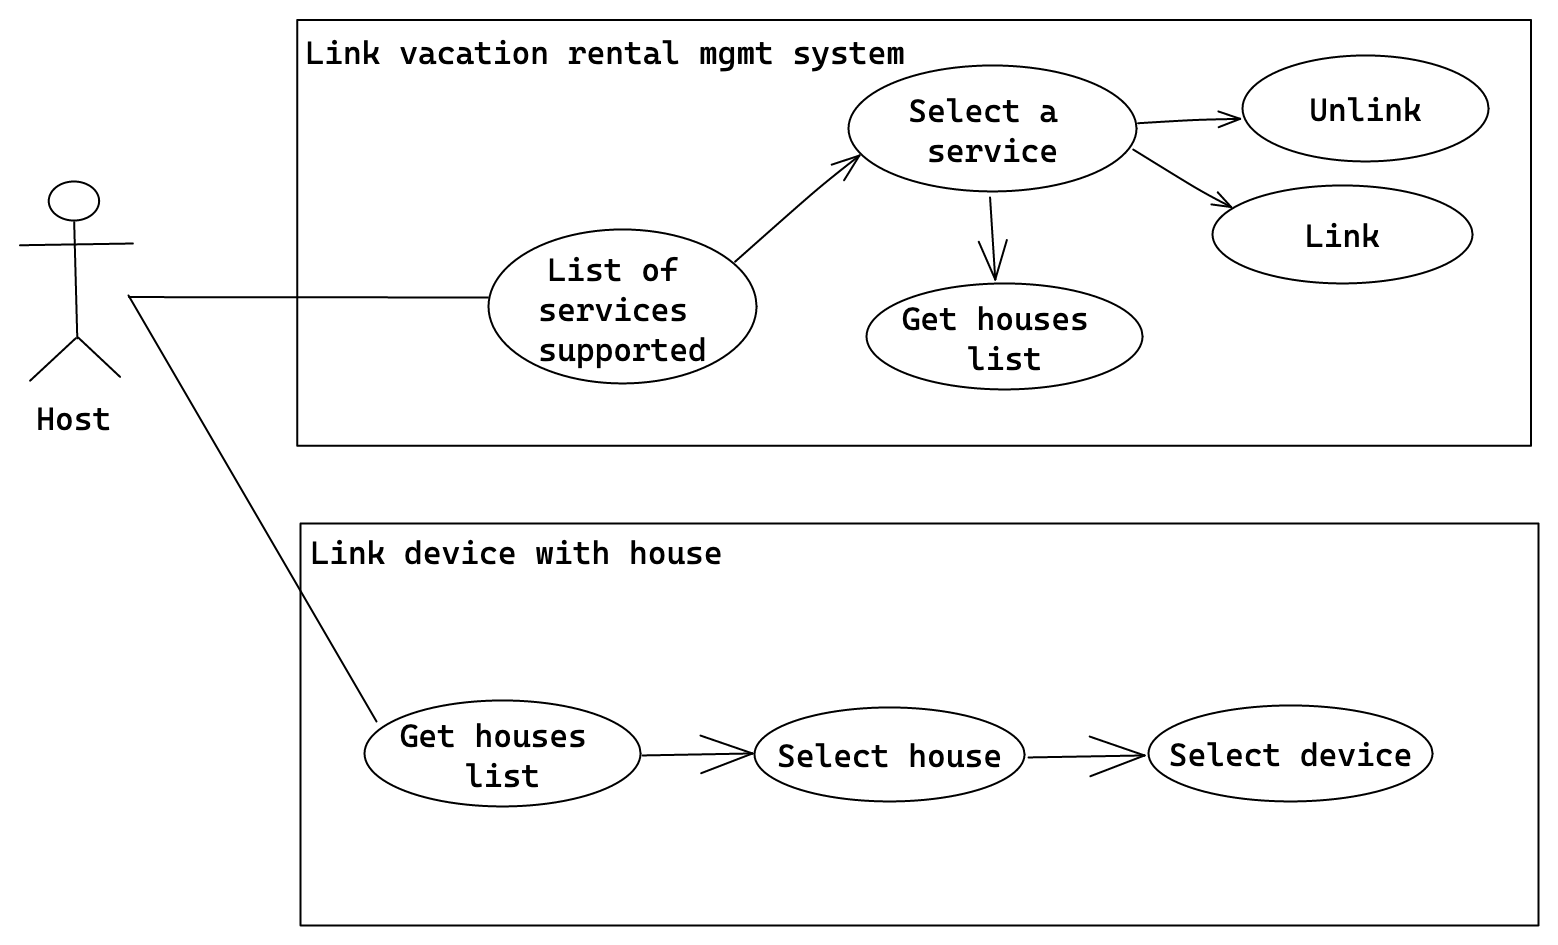
\includegraphics[width=0.8\textwidth]{figures/vrms.excalidraw.png}
    \caption{Vacation rental management system use case}
    \label{fig:vrmsusecase}
\end{figure}
Finally, to enable automatic key generation, the system must use the webhook of the vacation rental system management. As such, as in the smart-lock case, there is the possibility of linking and unlinking an external account, through the related authentication mechanism. This is actually an optional requirement; as such, the system can be designed without those particular features.

\subsection{Other diagrams}
During the analysis, some other diagrams were created, which can now be useful to understand how many parts of the architecture work.
\subsubsection{Create Key}
\begin{figure}[ht]
    \centering
    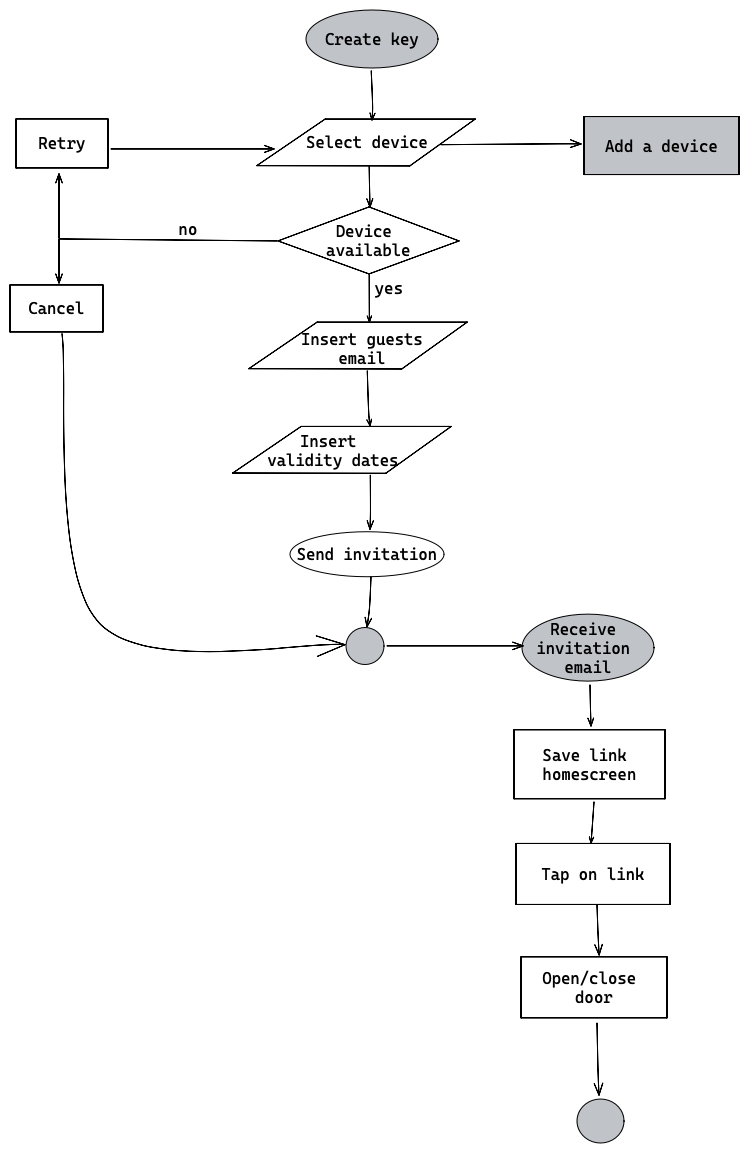
\includegraphics[width=0.6\textwidth]{figures/keyflow.excalidraw.png}
    \caption{Key creation flow diagram}
    \label{fig:keyflow}
\end{figure}
Key creation is a core feature of the application; therefore, we focus on the details of its steps. As we can see in the flow diagram in figure \ref{fig:keyflow} there is emphase on the initial check of the availability of the device. The importance of using a reachable smart-lock is fundamental, as such the host is always notified about the status of their devices.
In particular, we thought that a user should not have the possibility of creating a key on a non-accessible device.

\subsubsection{Add a Nuki account}
\begin{figure}[ht]
    \centering
    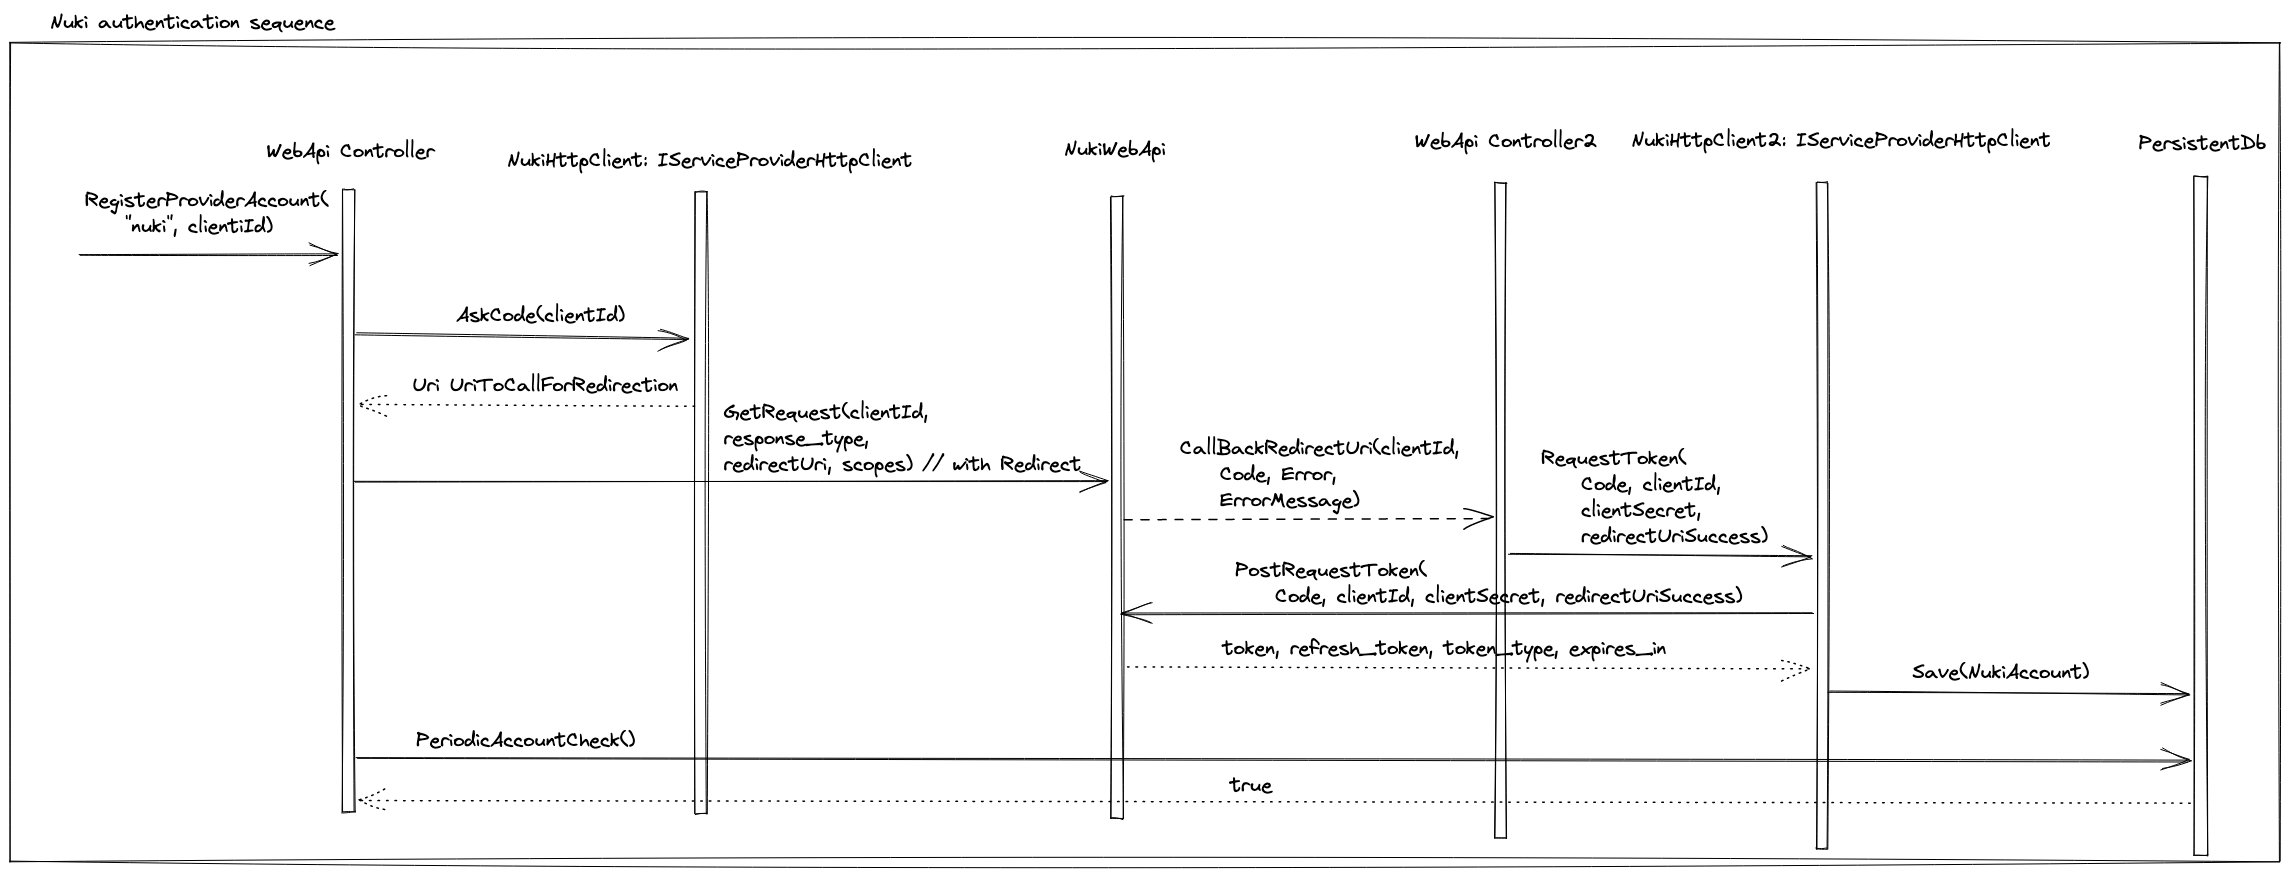
\includegraphics[width=\textwidth]{figures/nukiadd.excalidraw.png}
    \caption{Link a Nuki account sequence diagram}
    \label{fig:accountsequence}
\end{figure}
The link of a Nuki account that follows the OAuth2 authentication process was trivial during the design of the application. In particular, during the feasibility study, the initial test and the Proof of Concept implementation, as such we made a sequence diagram to clear up the entire flow. This process will be better explained in the next section \ref{sec:oauth}.

\subsubsection{Entities diagram}
Once determined the use cases and requirements, we proceeded with defining the entities involved in the application. An entity is any identifiable and separate object that is significant for the application. The diagram, in figure \ref{fig:entitiesdiagram}, defines which are the entities, their attribute and how they are related to each other. 
\\ This entity diagram refers only to the host, which is identified as \textit{user}. As we can see, a user can own more than one \textit{ProviderAccount} or \textit{RentProviderAccount}, which are abstractions of an external account, respectively, of a smart lock provider and of a vacation rental management system. Moreover, both of these entities are considered as interfaces with zero or one relationship between the main entity and its specifications. 
\begin{figure}[H]
    \centering
    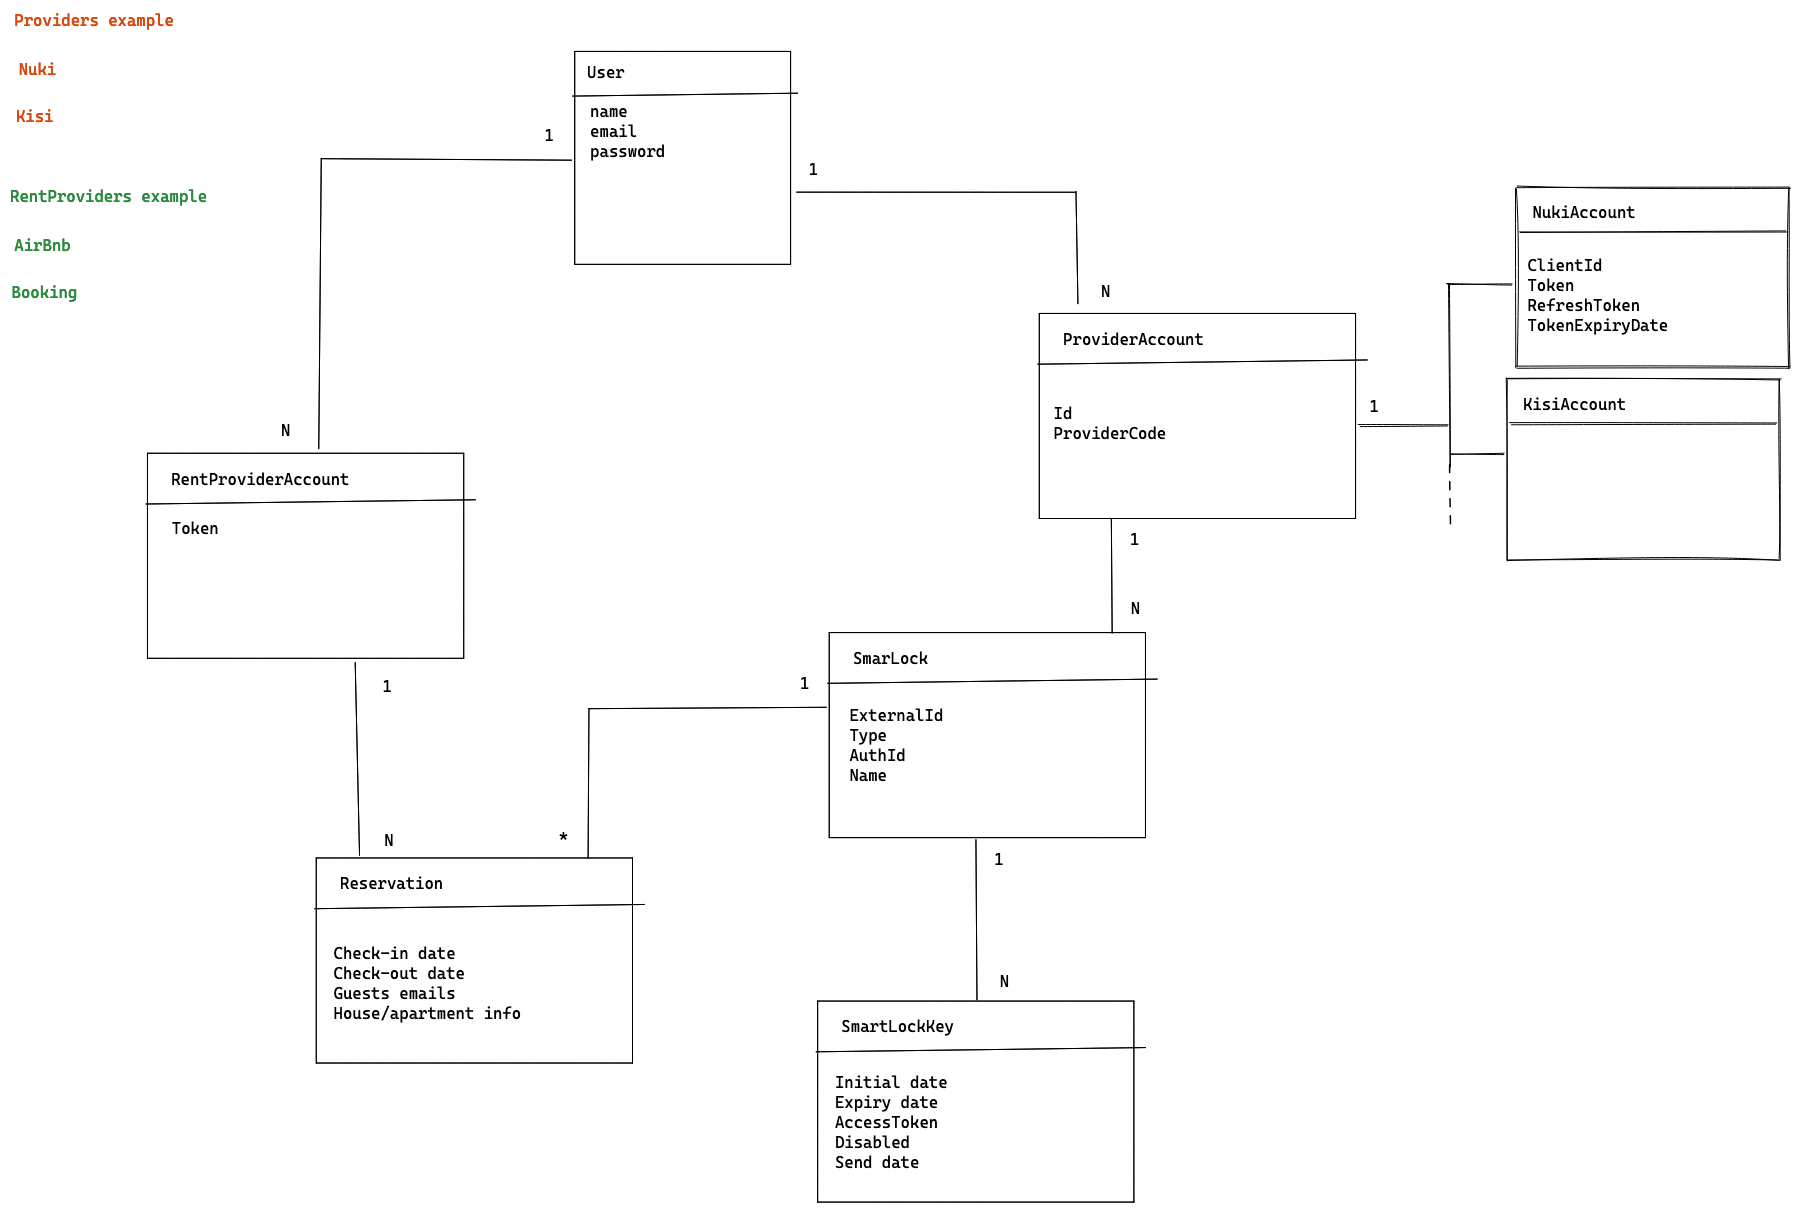
\includegraphics[width=\textwidth]{figures/entieties.excalidraw.png}
    \caption{The Kerbero entity-relationship diagram}
    \label{fig:entitiesdiagram}
\end{figure}

\section{Feasibility study}
While performing the requirement analysis, we conducted a feasibility study to check whether our assumptions were actually implementable with existing technologies. 
\\ The focus was, of course, on the state-of-the-art technologies involving smart-locks, which are already and extensively treated in the previous chapters. However, it was important searching and selecting the smart-lock solution, which could actually satisfy the use cases we had defined. 
\\ The most important feature a product must have is, of course, the availability of the public \acrshort{api}s. The integration of Kerbero with manufacturer software and systems was an essential precondition that we searched over all the alternatives taken into account. 
\\ Moreover, we searched for the characteristic of the product, the independence of the main operation from the manufacturer application and an integration with the already existing invitation system, which is translated in our project as the creation of virtual keys. 
\\ In light of this, a wide search on internet of the products was performed, which better fit the model we traced. In particular, we classified products according to the characteristic of our interest, as shown in the table \ref{tab:smartlockfeat}.

\begin{table}[ht]
    \begin{tabular}{|l|c|}
        \hline Host device Bluetooth pairing without app & C1 \\
        \hline System invitation acceptance without app & C2 \\
        \hline Possibility to Lock/Unlock without app & C3 \\
        \hline Must have to apply for more integration & C4 \\
        \hline Already offers an integration with a vacation rental management service & C5 \\
        \hline
    \end{tabular}
    \vspace*{0.3 cm}
    
    \begin{tabular}{|l|c|c|c|c|c|c|c|}
        \hline & Nuki & Kisi & Salto & Latch & Operto & Yale/August & Brivo \\
        \hline C1 & $\mathrm{x}$ & $\mathrm{x}$ & $\mathrm{x}$ & $?$ & $?$ & $\mathrm{x}^{**}$ & $\mathrm{x}$ \\
        \hline C2 & $\mathrm{x}$ & $\checkmark^{***}$ & \checkmark & $?$ & $?$ & \checkmark & \checkmark \\
        \hline C3 & \checkmark & \checkmark & \checkmark & $?$ & $?$ & \checkmark & \checkmark \\
        \hline C4 & \checkmark & \checkmark & $?$ & $\checkmark^{*}$ & $\checkmark^{*}$ & $?$ & $?$ \\
        \hline C5 & \checkmark & \checkmark & $\mathrm{x}$ & $\mathrm{x}$ & \checkmark & $\mathrm{x}$ & $\mathrm{x}$ \\
        \hline
    \end{tabular}
    \vspace*{0.3 cm}

    \small
    \begin{tabular}{c|l}
        \multicolumn{2}{l}{Legend:} \\
         \checkmark & Feature available \\
         x & Feature not available \\
         ? & No access to this information \\
         * & no access without \\
        ** & wi-fi only - need a code \\
        *** & with white labelling
    \end{tabular}

    \caption{Comparison between product of different manufacturer, related to some characteristics of interest.}
    \label{tab:smartlockfeat}
\end{table}
The choice of the first device to integrate in our system was relapse in the Nuki smart lock, the description of which is already widely covered in the chapter \ref{cap:three}. 

\subsection{The vacation rental management integration}
The integration with the vacation rental management systems are intentionally excluded from the mandatory requirements of the project, because of the difficulties of accessing their APIs. In particular, \gls{Airbnb} and \gls{Booking} \acrshort{api}s were considered the most used platform worldwide. We found that their APIs was selectively open, and as such if a developer wants to use them, he must perform a request to the vacation rental management system support service.
\\ Moreover, it is a common thought that Airbnb is very selective with companies asking for access to their APIs. As such, when a company wants to apply, it is suggested that they already have a working application to give as proof. 
\footnote{
\begin{quote}{From the Airbnb site: \href{https://www.airbnb.com/partner}{https://www.airbnb.com/partner}}
    "At this time, we are not accepting new access requests for our API. Our global team of partner managers will reach out to prospective partners based on the supply opportunity your business represents, the strength of your technology, and the ability to support our shared customers."
\end{quote}
}
Those are the reasons we decide to develop the application modularly, from the core features to the plugins for each of the providers. However, the main module of the application was only prepared to work without adding any integration with a vacation rental management system.

\section{Software design}
In this section, I would like to outline most of the design choices we decided to adopt to implement the previous detected features. For each of the following, a \acrshort{poc} was developed to prove the validity of the assumption and to test the features in a real world scenario. 

\subsection{Smart-lock keys design}
An essential decision during the design of the application was how to properly model the concept of virtual key. In the real world, keys are the only way to lock/unlock a door. We expect that this behavior remains invariant with the virtual model, as well. However, a virtual key has an important upcoming that the traditional key does not have: the possibility to be invalidate immediately. This benefit brings many others, such as the possibility to temporize the key or to give access to a person once and then revoke the permission. 
\\ Another important characteristic of the Kerbero keys is the ease of the use of guests. As such, the requirements we fixed for the keys were:
\begin{itemize}
    \item no mobile application to open and close the door;
    \item availability for mobile;
    \item security relying on a password.
\end{itemize}
Therefore, we decide that the key must be a public page accessible with a link and available only through the insertion of a keyword as a password, randomly generated by the application. The idea is that a guest receives a link to the virtual key page and a random password by email (fig. \ref{fig:keyfeat}). The guest is suggested to save the key link on the smartphone home and to keep the password safe and private.
\begin{figure}[ht]
    \centering
    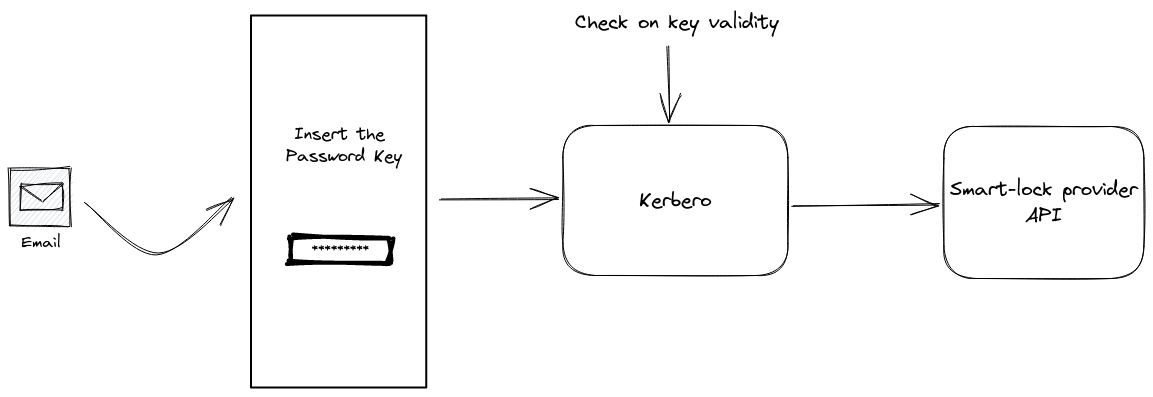
\includegraphics[width=0.9\textwidth]{figures/keyfeat.excalidraw.png}
    \caption{Key functional process}
    \label{fig:keyfeat}
\end{figure}
\\ This approach does not reach the security level of using a dedicated application, but is much easier to use for the end user, who does not have to download an application and create a new account. Moreover, the security level of the provider application rely on the use of a Bluetooth pairing between the devices, which assures that both of them are distinct entities that recognize each other. If the request is coming from the internet, this benefit is lost; the request is signed by the client ID of the application which is sending it, but the identity of the guest can not be tracked, except by the client itself. However, the smart-lock does not recognize information of this type coming from the client, as such that becomes useless. 
\\ Moreover, the non-usage of the official smart-lock application brings to others comedowns. Most of the features available through Bluetooth, such as auto-unlock or geo-fencing, are not usable through \acrshort{api}s. However, it is important to note that these features are mostly used in a smart house context, which is not our purpose. The design we proposed is guided by the assumption that an Airbnb host already knows what are the risks of giving the access to a stranger, as such, we premised that in the overall process mutual trust is involved.

\subsection{Smart-lock management}
Since the application is designed to operate with all the smart-lock through their \acrshort{api}s, the Kerbero specific model must be more generic than possible. In Kerbero the smart-lock data is not persistent, the information are fetched with the external API, in order to avoid out of sync and inconsistency. As such, most of the work of the plugin is to translate the information coming from the external APIs into a readable object for the Kerbero system.
\\ About the "writing" operations, such as the open and closed, keeping the object generic becomes more complicated. The process divides into various steps, as can be seen in figure \ref{fig:opensmartlock}. The logged in user has saved different credentials for each of the provider supported by Kerbero. As such, the request must provide \textit{Provider Identifier}, which serves the Kerbero component to switch between the right credentials and the repository to select. 
\begin{figure}[ht]
    \centering
    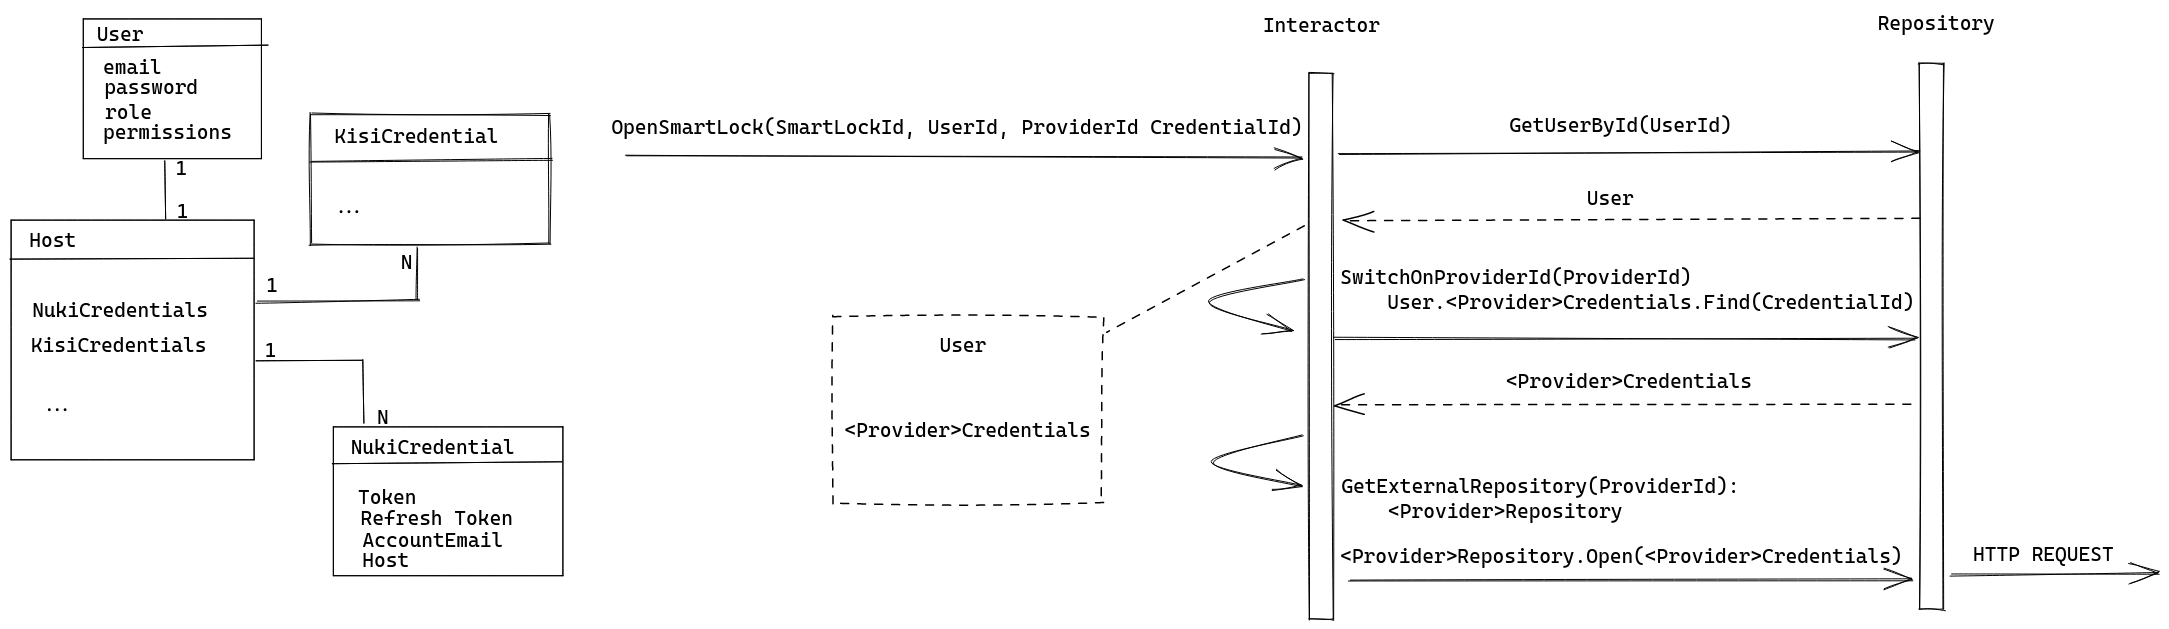
\includegraphics[width=\textwidth]{figures/open.excalidraw.png}
    \caption{A schema for opening a Kerbero smart-lock, an interactor (a method satisfying a use case) communicate con repositories on the data layer.}
    \label{fig:opensmartlock}
\end{figure}

\subsection{Application identity management}
In the section \ref{sec:actors}, we had given a hint of the authentication model through the specification of the actors involved. In particular, it was revealed that the host is the only role that must have a distinguished identity. As is said before about the keys, the guests do not need to identify themselves into the system, because they use keys which are not associated with any identity. 
\\ Therefore, the host needs an identity system that he can authenticate and, as a consequence, have access to the features of the application. The design of this type of functionality generates a lot of discussion and the choices we make here have involved the overall system architecture. The identity system we were looking for was not complicated; however, it needs the following properties:
\begin{itemize}
    \item one level permission for the user, which means that the application does not need to have different access level or locked features only for a specific type of user. This is a choice tight with the concept of ease of use outline in the requirements.;
    \item persistence of information related to the user;
    \item scalability oriented;
    \item email account confirmation.
\end{itemize}
The framework which grants to us this specification and the following authentication system is ASP.NET core identity, which will be described later in section \ref{sec:aspnetidentiy}.

\subsection{Cookies authentication}
The Kerbero client runs on a Web application which provides a Graphical User Interface (GUI) for the host. Moreover, there is a sever side application which performs the core actions. To maintain the authentication session, it was chosen to use browser cookies. They are managed in order to provide a user state both on the application side; therefore, providing a session for the client and a valid user identity on the server. 
\\ The operations on the cookies are simple and robust: the client sent the log in information to the server, the server checked the information, and if they are correct, it created a cookie which is attached to the response of the authentication request. The browser that receives the cookie in the header of the HTTP message saves the content in its immutable cache storage, called the cookie jar. As such, every time the client does a request, the cookie is attached, the server receiving the message checks the validity and the content of it.
\begin{figure}[ht]
    \centering
    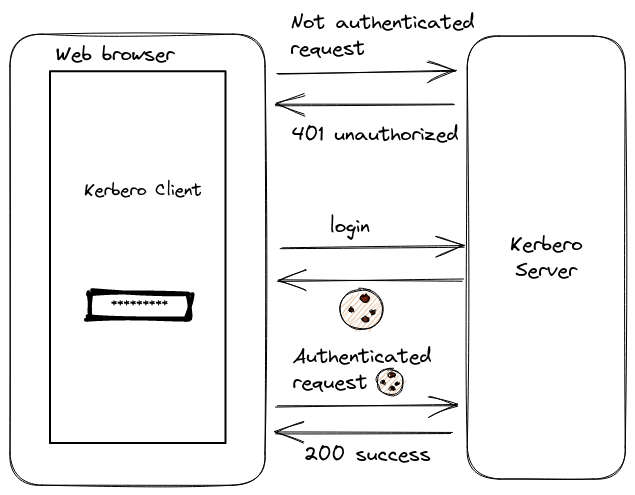
\includegraphics[width=0.6\textwidth]{figures/cookiesflow.excalidraw.png}
    \caption{The cookie session and authentication management.}
    \label{fig:cookieflow}
\end{figure}

\subsubsection{Cookies specification}
In order to better understand the reason for the choice of cookie authentication, it is important to know their specifications.
\\ Cookies are born as a way to pass a small piece of information from the client to the server and vice versa. As such, the purpose is to create a shared state between the two actors over the HTTP protocol. 
\\ By default, the cookie was not built for security; it guarantees neither confidentiality nor integrity of the transferred data. However, it is worth mentioning two attributes of the cookie: \textit{Secure} and \textit{HttpOnly}.  \textit{Secure} attribute limits the use of a cookie to only secure channels. As such, the client attaches the cookie only when the request is over \acrshort{tls}. Note that, while this protects the confidentiality of the cookie, it does not protect its integrity if an attacker sends the request from a secure site. The second attribute, \textit{HttpOnly}, limits the cookie to be used only on HTTP request, which means that it cannot be modified by the JavaScript of the browser and, as such, it can only be writable on the server side\cite{8392612}. Thanks to this mechanism, the cookies can only be saved in the browser, as such the ones created by the client and attached to an HTTP request are ignored by the server when received. As a consequence, the unique flow available to manage them starts from the server, which attaches the cookies he needs on the HTTP request and the browser receiving them has to store in the cache. Then, it can resend their content with the following request. As such, the cookie jar, if correctly managed from the server, is read-only on the client side. As a result, the server is considered a trustworthy entity that can manage the state of the browser. 
\\ Therefore, the client is resistant to many attacks related to cookies, in which malicious code writes a copy of an existing cookie, to emulate authentication, for example. If the cookie is properly configured, those attacks cannot be launched from the client side, by injecting JavaScript code. This is avoided by the fact that, due to the \textit{HttpOnly} attribute, JavaScript scripts can access read-only cookies.
\\ Moreover, the update process of a cookie grants a low level of integrity. In fact, all cookies are identified by a key that provides uniqueness. If a new cookie with the same key and different content is received by the browser, he must update the existing one with the new information. 
\\ An additional security layer is granted by the \textit{SameSite} attribute. The same-site cookies are a relatively new HTTP specification, which provides to the client a way to decide which cookies can be sent in the request to the server.  \textit{SameSite} attribute was specified to avoid cross-site request forgery attacks, which are particularly dangerous to security\cite{ietf-httpbis-rfc6265bis-11}. This type of attack affects authentication; in fact, if an attacker manages to provide a stolen cookie, he can set the cookie with a malicious application and call the real server. As such, the real server recognizes the cookie as valid, and it provides a valid response. The same-site cookie prevents that with an URL restriction, which limits the cookies to the origin site with a URL domain check. \textit{SameSite} can be set with three different values:
\begin{itemize}
    \item \textit{None}, which disables the whole protection mechanism;
    \item \textit{Strict}, which defines that the client can send the cookie only to the origin site;
    \item \textit{Lax}, which is similar to strict, but the client can send the cookie even if he is on another domain, reached after a redirection from the origin site. 
\end{itemize}

\subsubsection{Why cookies over Bearer token}
As we have seen so far, cookies are strongly bound to browser technology. As such, they cannot be used for other types of client, like a mobile or desktop application. Therefore, a bearer token solution, maybe combined with an OAuth2 authentication flow, seems to be a better solution in the context of an REST API. 
Moreover, bearer tokens are generally more secure than cookies, since they are not stored on the client machine and are less vulnerable to tampering. However, they can be more difficult to use since the server must keep track of the tokens and implement additional security measures to prevent unauthorized access. Furthermore, cookies technology, with \textit{HttpOnly}, \textit{SameSite} and \textit{Secure} attributes, improves a lot in recent years, reaching almost the same security level of the bearer token.
\\ The two benefits we recovered from using the cookies were:
\begin{itemize}
    \item they are lightweight and more informative;
    \item completely managed by the browser and the server side framework;
    \item they are valid for the entire session, until the browser wipes the cache.
\end{itemize}
It is important to note that most complex applications usually combine these two methods. The reason is that a large application has many different clients. If the client is a web browser it is commonly used the cookies solution; however, if the client is a dedicated mobile or desktop app, the bearer token is the only way. Therefore, Kerbero is now implementing only cookie authentication, but is already prepared for the future addition of another authentication method.

\subsection{OAuth2 authentication flow management}
\label{sec:oauth}
During the analysis, we noticed that access to the smart-lock service \acrshort{rest} \acrshort{api}s is almost always protected with an OAuth2 authorization flow. OAuth2 is an authorization framework that enables external applications to obtain access to a user account linked to an HTTP service. It is usually used when a service is integrating an external one; as such, the first one needs to ask the permission to the user of the second. As such, OAuth2 works by delegating user authentication to the service that hosts the user account, in order to give the access permission to the application requesting the integration.
\\ The roles involved in the process are:
\begin{itemize}
    \item the resource owner, which is the entity that is responsible of the user account;
    \item the client is the application which requires the resource;
    \item the resource server, which is the place where is located the data the client is looking for;
    \item the authorization server, which is the authority managing the authentication and the permission access to the resource.
\end{itemize}
\begin{figure}[ht]
    \centering
    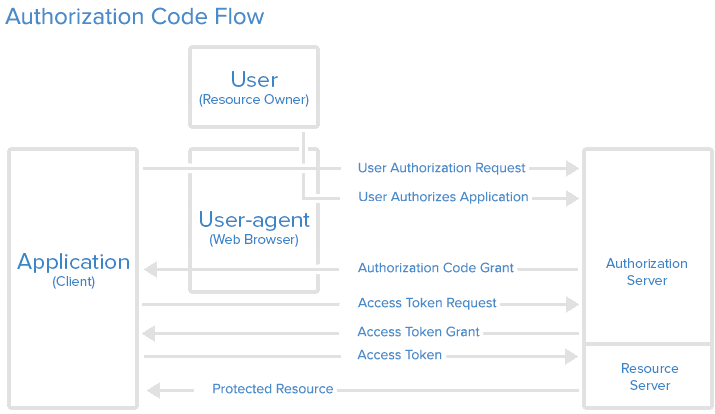
\includegraphics[width=0.7\textwidth]{figures/auth_code_flow.png}
    \caption{OAuth2 protocol flow.}
    \label{fig:oauthflow}
\end{figure}
As we can see in the figure \ref{fig:oauthflow} the components interact with each other, in order to provide the client with the possibility of reading or writing the protected resource, in the form of an access token. \cite{anicas_2014}
\\ In order to represent a valid application, the client must register with the service. The common way is to provide the client with a \textit{client identifier} and a \textit{client secret}, which must be exchanged during the authorization phase. 
\\ From the client's perspective, the authorization process requires two phases.
\begin{itemize}
    \item First of all, the client must ask the user permission to use the information in his account. In order to do so, the resource owner must expose an authentication service dedicated to the OAuth2 service. The client user is commonly redirected to the authentication service page of the resource owner, where he must log in and accept the read or write permission request to the resource. Once the user completes this procedure successfully, the authorization server returns a code which is not yet the access token.
    \item In the second phase, the client must request the access token to the authorization server. The request is performed using the code given in the previous phase, which is temporary and usually single-use. The response of the authorization server contains the access token, which is the bearer token, and the refresh token, which is used, indeed, to update the access token when it expires. 
\end{itemize}
One of the most difficult challenges faced during the design of the application is the integration of the OAuth2 authentication flow with our authorization system. The problem relies on the end of the first phase, when the authorization server calls the client with a callback to provide the code. The endpoint exposed by the client must be anonymous, that is the server can be not authenticated to call it.
This choice is mandatory, since the authorization server does not know anything about the client authentication system. However, when the client endpoint computes the information it has no clues about the identity of the user who has started the OAuth2 flow. 
\\ In this case, the cookie authentication flow is handy, in particular, the \textit{SameSite} attribute \textit{Lax}. This attribute solves the problems applying a same-site cookie policy less rigid, as such the authentication cookies are sent back from the user-agent (in fig.\ref{fig:oauthflow}) to the client, which in this case is Kerbero. As a result, the client can use the cookie to authenticate and retrieve all the information about the user. 
\\ It is important to note that this solution can only be implemented with cookies. As such, being only available within the browser, the only possible way to manage OAuth2 authentication seems to be restricted to web applications. However, most of the development framework, like Java/Kotlin Android, Swift, etc., has libraries which can typically manage the flow with a redirect to a web view.

\subsection{Error management design}
\subsubsection{HTTP errors}
The error management was another challenge during application design. It is important to assume that the application is client-server. The client, as we already mentioned, is a web application, while the server is a \acrshort{rest} \acrshort{api}.
\\ The REST API typically responds to client requests with an \acrshort{http} response, which contains a JSON object, which is a standard data format, used to define data objects that can be read by different languages and frameworks. Inside the JSON we usually find couple formatted as keys and values. In case of error, the HTTP message contains a specific field called response status code, which contains a number indicating the a standard HTTP error. 
\\ Kerbero uses a message-status code approach, as such the client everytime receives an error as response, the latter will contain both a proper status code and a message inside the JSON object. As such, the client has a filter which determines if the error has to be shown as a pop-up or managed internally.

\subsubsection{Language exceptions}
About the exceptions, the strategy applied was "catch everything". The server side approach is translated in functional, as such every source of error is closed in a try-catch block. Therefore, the catch encloses the return object of the function in a specific result type. This approach has proven to fit particularly well, with the architectural choices we made for the application, treated deeply in section \ref{sec:architecture}. In general, we can say that a functional approach grants modularity because force the error to be managed in the function scope. Moreover, the object result can contain more than one error, as such it can be more informative of a managed exception. However, the correctness of this approach depends a lot on the implementation and the responsibility relies on the developer. Moreover, many server-side frameworks offer an automatic way to filter and return HTTP status code based on the type of exception returned. However, this approach most of the time does not give the possibility of returning other information, such as a message, which brings this feature out of our scope.   

\subsubsection{External errors}
The last design choices on error management are related to external services. Kerbero is implemented to communicate with external APIs, as such it needs a well design way to handle the errors coming from them. As we said in the previous section, all the exceptions are wrapped in a try-catch and translated into a result object with an error field. This approach is used with external errors too, in fact the client HTTP is designed to throw exception in case of status code different from success (i.e. 2XX). Then, the exception is caught and wrapped in a result object, including a custom error or a list of custom errors. This approach is more flexible than the exception propagation, because it allows the server to decide which errors have to be managed or ignored.

\section{Project plan}
In this section, we will discuss architectural choices and a brief description of the technologies involved in the project. These choices were particularly crucial during the development of the application. Architecture, in particular, was difficult to design because we had to take into account many different factors. At first sight, from the requirement analysis it seems that there are not many problems that require complicated solution. However, Kerbero has a scaling nature; in fact, the goal is to implement more and more plugins in the future, in order to give support to new smart-lock devices. As such, the modularity and, as a consequence, the dependencies question was crucial on the application designing. 

\subsection{The Kerbero architecture}
\label{sec:architecture}
In order to provide a robust split between the user interface and the business logic, Kerbero is divided into a client-server application (fig. \ref{fig:kerberoarchitecture}). The reasons for this choice are based on allowing the application to implement different types of client. If, in the future, the resources will allow an implementation of a mobile application, the architecture is studied to give the possibility to be upgraded with only few changes server-side.
\\ The server-side is also designed as modular as possible, dividing layers and business logic in low code dependency sections. Moreover, these modules are organized inside the architecture to have isolated communication with all the external resources. This will be discussed in depth in the next section. 

\begin{figure}[ht]
    \centering
    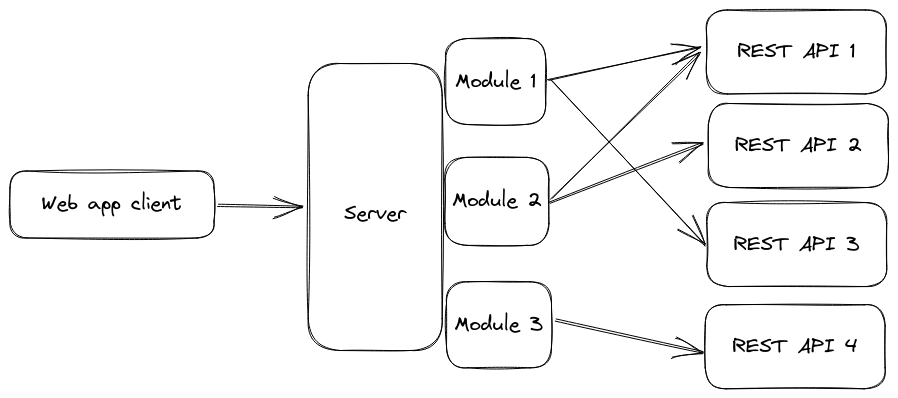
\includegraphics[width=\textwidth]{figures/architecture.excalidraw.png}
    \caption{High level architecture of Kerbero}
    \label{fig:kerberoarchitecture}
\end{figure}

\subsubsection{The clean architecture}
\paragraph{The specification}
As we said previously, the application must implement software that is as less dependent as possible. As such, the choice of architecture falls on the Clean architecture. 
\\ The Clean architecture, also known by the name Onion architecture, is not a properly defined standard pattern, but a collection of best practice and rules to apply to achieve separation of concerns\cite{uncle_bob_2012}. This allows the architect to produce a system which is:
\begin{itemize}
    \item independent of frameworks and existing library;
    \item independent of any external agency, database or UI;
    \item testable, thanks to the low dependency between the components.
\end{itemize}
The main rule to follow in Clean architecture is \textit{Dependency rule}, which says that all dependencies of the source code can only point inward. As such, we can see the system as a set of concentric circles in which the inner ones do not know anything about the outer ones. 
\\ In the clean architecture the \textit{Entities} play an important role. They are object containing methods, attributes, or data structures that represent system-wide business rules. The latter are the high-level behaviors of the application, which represent the smallest and least dependent unit of logic. Furthermore, entities should not be affected by operational changes. As such, they are inserted in the inner circle of the architecture. 
\\ The entities are wrapped by the use cases, which represent the application specific business rule. They should encapsulate exactly the use cases defined in the requirement analysis.
\\ The following circles are out of business logic and have to deal with external resources. As such, the first layer we encounter is the interface adapters, which translate the data into a convenient format for the underneath layers.

\paragraph{The implementation}
Following the Clean architecture rules, the system obtained results to be robust and with a low level of dependencies. The architecture is divided as we can easily see in figure \ref{fig:cleanarchitecture}. 
\\ We managed to combine the entities and use cases in a single module, which is called \textit{Domain}. The unusual thing in this architecture is the separation of the identity module from the business logic of our application. This was forced by the fact that this library was already implemented and we simply imported it inside the project with few modifications. The library was not implemented in clean architecture, as such, in order to not disrupt the dependencies, we managed to put it as inner circle next to the Domain layer, however, without any dependency with it. 
\\ The middle circle contains the infrastructure level. As such, here we can find the interface to the external resources and the mappers, which manage to translate the data from and to the inner circle. Finally, the outermost circle physically represents external resources, such as the database, external APIs, and the web application, which is the user interface.
\begin{figure}[ht]
    \centering
    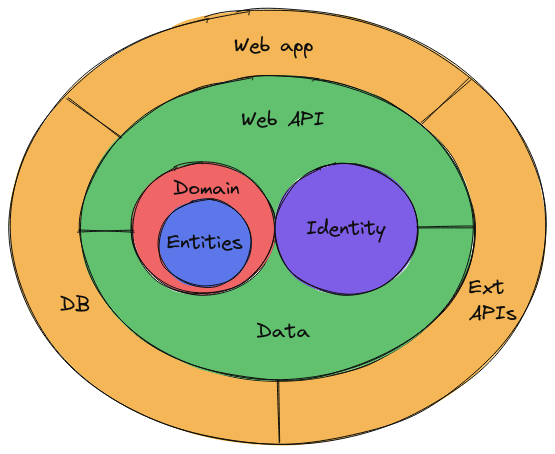
\includegraphics[width=0.65\textwidth]{figures/cleanarchitecture.excalidraw.png}
    \caption{The Kerbero components organized with the clean architecture}
    \label{fig:cleanarchitecture}
\end{figure}

\paragraph{Evaluation of the architecture}
After the implementation of the architecture, the dependencies schema appears to be as in the figure \ref{fig:dependenciesschema}. \\
\begin{figure}[ht]
    \centering
    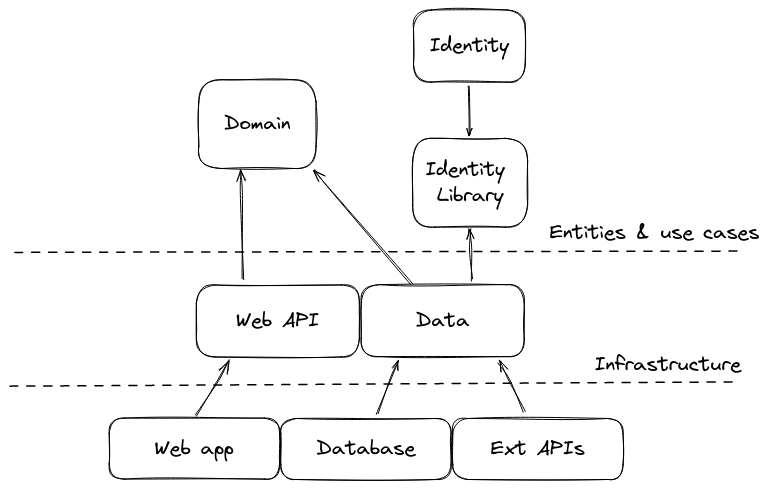
\includegraphics[width=0.70\textwidth]{figures/dependenciesschema.excalidraw.png}
    \caption{The dependencies schema of Kerbero.}
    \label{fig:dependenciesschema}
\end{figure}
Following the previous rules was not that easy, in fact, the figure \ref{fig:cleanarchitecture} represents the last version of the architecture to which we came. As such, the initial version of the architecture was substantially different from the latest one. The analysis and the feasibility study were not enough to determine the final architecture a priori. This is caused by the rigidity of \textit{Dependency rule}, which sometimes does not conform to the best practices of external libraries or frameworks, as it declares. In fact, it turns out that if a library needs to be inserted inside an internal circles (which in most of the cases must be avoided), then many problems emerge, especially if the latter does not implement the clean architecture first. As such, during the development can happen that the library, chosen as data access framework, needs a dependency on an object in order to work and the developer must move this object from an inner circle to an outer one; or he must create a copy of that class inside the module, and, as a consequence, he has to code the mappers and the utilities for that specific unit. As such, Clean architecture requires a large codebase to be implemented in a real-world scenario, with respect to the alternatives, such as the layered or the monolithic architecture. Moreover, we found that it was not that easy to read by an external developer, as such the components need a detailed description first.
\\ However, the resulting application turned out to be, as expected, modular and with a low level of interdependencies between its components. This was a requirement for the scalability of the application, but the latter was not the only benefit. The application tests were easier to implement than expected, even the integration and end-to-end tests. Also, the debugging of the application was helped by the modularity, thanks to the ease of finding the error in isolated components. 

\subsubsection{Project structure and component naming}
The architecture, finally, has determined the structure of the project. As such, from there is possible to understand even better the concepts outline in the previous sections. Following a partial directory tree of Kerbero. 
\begin{scriptsize}
\setlength{\DTbaselineskip}{8.5pt}
\dirtree{%
 .1 .
 .2 docker-development-db.
 .2 web-api.
 .3 src.
 .4 Kerbero.Data.
 .5 Common.
 .6 Context.
 .6 Helpers.
 .6 Interfaces.
 .6 Repositories.
 .5 Migrations.
 .5 <Module Name>.
 .6 Dtos.
 .6 Entities.
 .6 Mappers.
 .6 Repositories.
 .4 Kerbero.Domain.
 .5 Common.
 .5 <Module Name>.
 .6 Errors.
 .6 Interactors.
 .6 Interfaces.
 .6 Models.
 .6 Repositories.
 .6 Utils.
 .4 Kerbero.Identity.
 .5 \dots.
 .4 Kerbero.Identity.Library.
 .5 \dots.
 .4 Kerbero.WebApi.
 .5 Controllers.
 .5 Dtos.
 .5 Exceptions.
 .5 Extensions.
 .5 Mappers.
 .3 tests.
 .4 \dots.
 .2 web-app.
 .3 \dots.
}
\end{scriptsize}
\hfill \break
From this directory tree we can also notice the naming of the component in the architecture. Starting from \textit{Domain}, we can identify the clean architecture entities and use cases, respectively, as \textit{models} and \textit{interactors}. Then, there are the errors, the interactors and the repositories interfaces, useful to be used with the Dependency Injection (DI).
\\ Inside the \textit{Data} component we identify some of the classes and concepts related to external libraries, such as the \textit{Context} of the Entity Framework core tool. Specific of this layer is the implementation of the repositories, which are specific for each entity and provide the basic methods to manage them, as such the creation, reading, updating and deletion (CRUD). Moreover, there is a strangeness, which is the presence of \textit{entities}. The latter are not to be interpreted in the clean architecture way, but they are named according to the naming of the library with which they are used, EF core. Both in the Data and WebApi layers, there are \textit{dtos} and \textit{mappers}. The first one are the Data Transfer Objects (DTOs), which represent the data structure entering and exiting the system. The characteristic of this type of data is the possibility of being serialized and deserialized the object, in order to fit in an HTTP message as a JSON. Finally, to deal with the different forms that the same data type can have (DTO, entity, or model), there are \textit{mappers}, which have the task of transforming the object from one type to another, modifying and filtering their attributes.

\subsection{Workflow, versioning and conventions}
The implementation of the application never reached the production state, therefore, it remained in a development state for the duration of the project. As such, we needed only two types of environment in which run the application. We used a workbench in which we can experiment the technologies and test the integration between the components, as such here we used to build Proof of Concept software. The other environment is the development one, which includes a database on a virtual machine and the client-server architecture, which run with ad hoc scripts on the localhost.
\\ While the first environment was not versioned, the development environment is traced in a Version Control System. In particular, we use Git and Github to maintain a shared and remote repository for our codebase. Moreover, we used branching, rebasing and merging, in order to manage the concurrent and parallel development of features. In particular, there were three types of branch: \textit{master} contains the most stable and reviewed code; the \textit{feature} branches, which were used to develop a new module starting from the master or another feature branch code; and \textit{fix} branches, which contain little, but disruptive, modification, aimed at solving bugs or errors.
\\ Github has played an important role in the workflow during the development of the application. In particular, we exploited the Pull Requests (PR) feature. A PR is a merging request of a non-master branch into the master one. The importance of requesting first relies on the code that, before becoming part of the codebase, must be reviewed. Reviews were an important part of the project implementation phase. Moreover, Github offers other services, such as the possibility of launching actions on code pull, such as building and test commands. This grants having a working code in all branches. 

\subsection{The client architecture}
The client of the application is developed as a Single Page Application (SPA). A SPA is a web application or website that loads a single HTML page and dynamically updates the content as the user interacts with the application. It is designed to provide a smooth user experience similar to a traditional desktop application. SPAs are built using client-side JavaScript frameworks, such as Angular, React, and Vue, which allow them to update the content dynamically without having to refresh the entire page. When a user interacts with the application, the JavaScript framework updates the necessary parts of the page rather than loading a new page from the server. This results in a faster and more responsive user experience, since the application does not need to reload the entire page every time a user takes an action. SPAs typically use a routing mechanism to handle different URLs and will update the content based on the URL. They usually communicate with the server using APIs and JavaScript libraries, such as Axios or Fetch, to retrieve and update data. Kerbero uses a wrapped HTTP client around the Fetch library.
\\ One of the main benefits of SPAs is that they can provide a smooth user experience, with fast and responsive navigation, similar to a traditional desktop application. They also reduce the amount of data transfer between the server and the client, which can improve the performance of the application. However, one of the main challenges of SPAs is that they are not as SEO-friendly as traditional web applications, as search engines may have difficulty indexing the dynamic content of the application. Additionally, if the JavaScript code fails to load or execute correctly, the SPA may not be able to function at all. This limitation was taken into account before choosing this approach. In fact, we think that, like many other web applications, Kerbero does not need the search engine indexing the site; moreover, the problem can be bypassed easily with a workaround, such as linking the application from an indexed presentation page.

\subsection{Tests and security}
Most of the application was implemented using Test-Driven Development (TDD). The TDD is a software development process that involves writing automated tests for a specific feature or behavior the actual implementation. The tests are then continuously run to ensure that they fail until the feature is not completely implemented. When the tests are passed, it means that the feature is ready and that the developer can refactor its code to make it more efficient and readable. This process helps to ensure that the code is thoroughly tested and that the new changes do not break existing functionalities. It also encourages a more modular and flexible design, as developers are forced to think about how their code will be used and how it will interact with the other parts of the system.
\\ We focus, in particular, on server tests, which are of three types: unit tests, integration tests, and end-to-end tests (e2e tests). Unit tests were organized as a mirror of the source code directory. As such, all methods and functions are designed and tested before implementation following the TDD process. 
\\ The integration tests ensure that developers understand that all modules and layers communicate correctly with each other, while the end-to-end managed to test an entire feature from client input to response. 
\\ Testing was also designed to improve the security aspects, particularly those that involve authentication. During the end-to-end tests, for each of the actions exposed by the endpoint, it was verified that request with not valid cookies does not pass the identity controls, acted by the framework library. 

\subsection{Technologies and frameworks}
The committer did not imposed any limitation about the technologies to use during the implementation. As such, having this freedom, we managed to choose the best frameworks and libraries that fit the requirements of the application. This process involves many elements and, as such, takes a significant part of the scheduled time for the application development. In fact, for each of the following frameworks, a PoC was produced first, and then an evaluation, to better understand which combination of them can generate an application with such designing choices. 

\subsubsection{.NET and ASP.NET core}
About the implementation of the application server and the web API, .NET was chosen a framework maintained and developed by Microsoft. .NET is a free, open source, cross-platform framework for building various types of applications, including web, mobile, desktop, gaming, and IoT. It includes a large library of pre-written code, a common runtime environment, and a set of tools and languages that can be used to build and run applications. Some of the languages that can be used with .NET include C\#, F\#, and Visual Basic. The .NET framework supports multiple operating systems such as Windows, Linux, and macOS. 
\\ Kerbero was initially be implemented with .NET 6, but during the development we found out that many features of the just released .NET 7 might be useful to us. As such, we managed an upgrade rollout of the application, upgrading the associated libraries as well.
\\ The specific framework used to develop the web API was the ASP.NET core. ASP.NET is part of the .NET platform and is designed to be lightweight, high-performance, and modular. It provides a number of features that make it well-suited for building web applications, including support for routing, middleware, persistence and dependency injection, as well as built-in support for security features like authentication and authorization. One of the main benefits of ASP.NET Core is its ability to be hosted in different ways, such as IIS, Apache, or self-hosting. Additionally, it provides a flexible pipeline for handling requests and responses, which allows developers to easily add custom middleware and services to handle specific functionality. ASP.NET Core is designed to be highly performant, scalable, and easy to test, and it can be used to build a wide variety of web applications, including web APIs, MVC web applications, and the one of our interest: SPAs.

\paragraph{The dependency injection}
A feature that helps in the implementation of the clean architecture is the Dependency Injection (DI). The DI is a design pattern that allows a class or component to receive its dependencies from an external source, rather than creating them internally or hard-coding them. These dependencies are typically services or objects that the class needs to perform its intended function. The key benefit of using dependency injection is that it promotes loose coupling between classes, making an application more flexible, maintainable, and testable. When classes are loosely coupled, they can be easily replaced or modified without affecting other parts of the application. This makes it easier to add new features, fix bugs, and improve performance.
\\ One way to implement DI in .NET is to use constructor injection. This involves injecting the dependencies of a class through its constructor, allowing the class to use the dependencies without having to create or manage them. For example, using the built-in DI feature in .NET Core, you can register a service and its dependencies in the \textit{Startup} class and then use the service in a controller by injecting it through the constructor.
\\ Another way to implement DI in .NET is to use property injection. This involves injecting the dependencies of a class through its properties, allowing the class to use the dependencies without having to create or manage them.
Overall, the basic steps to implement DI in .NET are:
\begin{itemize}
    \item create an interface for the service that you want to inject; 
    \item create a class that implements the interface;
    \item register the class and its dependencies in the container;
    \item inject the service into the constructor or property of the class that needs it.
\end{itemize}    

\paragraph{EF core}
Moreover, we managed to choose a framework that allows abstract database management, integrated with the .NET framework. As such, the choice has been left to the EF Core.
Entity Framework Core (EF Core) is an open source and cross-platform Object-Relational Mapping (ORM) framework for .NET. In particular, it enables developers to work with relational data using domain-specific objects, and eliminates the need to write a lot of low-level data access code.
\\ EF Core provides a set of APIs that allow developers to interact with a database using C\# code, rather than writing raw SQL statements. It automatically generates the necessary SQL commands based on the C\# code and the database schema, and maps the results to the appropriate domain objects.
\\ EF Core also provides a powerful querying capability, allowing developers to use LINQ (Language-Integrated Query) to write type-safe, composable and expressive queries in C\#. It also supports lazy loading, change tracking, and caching, which makes it easy to work with large data sets.
\\ EF Core can work with different databases such as Microsoft SQL Server, MySQL, SQLite, PostgreSQL, and more through different providers, making it versatile and can be used in different types of project.
\\ One of the key features of EF Core is its flexibility and ability to work with different data access scenarios. It can be used in server-side applications as well as in client-side applications (desktop and mobile). It also supports different deployment scenarios, such as on-premises and cloud-based.

\paragraph{ASP.NET core identity}
\label{sec:aspnetidentiy}
For identity management, we integrate an existing project, which is a personalized version of the ASP.NET core identity library. As such, we make use of this wrapped version and adapt it to our purposes. ASP.NET Core Identity is a membership system that allows you to add authentication and authorization functionality to your ASP.NET Core web application. It provides a set of APIs and services for managing users, roles, and claims, and is built on top of the ASP.NET Core framework. ASP.NET Core Identity allows you to easily create user accounts and authenticate users in your application. It supports different types of authentication, including cookies, JWT tokens, and external providers like Google, Facebook, and Microsoft. It also provides built-in support for two-factor authentication, password hashing and salting, and account lockout policies. ASP.NET Core Identity also provides a way to manage users and their roles in your application. Provides a built-in user store that supports basic user management functionality, such as creating, updating, and deleting users. It also allows you to define and manage roles and assign users to specific roles.
Another important feature of Identity is claims-based authentication, which allows you to add additional information about a user, such as their name, email, and address, and use this information to make authorization decisions in your application.
\\ While role management was not part of our scope, claims allow us to save user information and use it to perform our authentication checks. Moreover, ASP.NET Identity provides a testable process for implementing email confirmation of an account, which was particularly useful.

\subsubsection{PostgreSQL}
For the persistence it was selected PostgreSQL, due to its renown quality, such as stability, robustness, and feature richness. It is often used for web and enterprise applications, as well as data warehousing and analytics workloads. PostgreSQL supports a wide range of data types, including text, numbers, dates, and binary data, and also supports advanced data types such as arrays, hstore (a key-value store) and JSON. It also supports full-text search and GIS (Geographic Information System) data types. Additionally, it has a large number of built-in functions, operators and aggregates. PostgreSQL supports multi-version concurrency control (MVCC), which allows multiple transactions to access the same data simultaneously without conflicts. With respect to performance, they have particular impact features such as point-in-time recovery, hot standby, and logical replication, making them a suitable option for large-scale, high-availability systems. Moreover, PostgreSQL is known for its robustness and stability, and it is widely used in production environments, it is also a good option for large-scale and complex projects, it is supported by many operating systems, and it can be easily integrated with other software and tools.

\subsubsection{Vue.js}
The Single Page Application was developed with Vue. Vue.js is an open-source JavaScript framework for building user interfaces and single-page applications (SPAs). It is known for its simplicity and ease of use, making it a good choice for developers who are new to JavaScript frameworks. It uses a template syntax that allows you to declaratively render dynamic data into the DOM, making it easy to understand and debug the application. It also supports a component-based architecture, allowing developers to create reusable and composable UI components. Vue also provides a powerful set of directives and built-in directives that allow you to easily manipulate the DOM, listen to events, and handle form inputs. It also provides a centralized state management system called Vuex, which makes it easy to share data between components and manage the application's state. Vue is also known for its flexibility and adaptability, it can be easily integrated with other libraries or existing projects, it also has a large and active community, which provides many resources such as tutorials, plugins, and packages.